% ============================================================
%  QCE26 Paper -- IEEE Quantum Week 2026 (Toronto, Sep 13-18)
%
%  Target length (supervisor): ~6 pages + 1 page references.
%  Class: \documentclass[10pt,conference]{IEEEtran} (no compsoc).
%
%  Structure: this main file only wires things together. Packages
%  and macros live in preamble.tex; each section, figure, table and
%  algorithm is a separate file under sections/, figures/, tables/,
%  algorithms/ and is pulled in with \input.
% ============================================================

\documentclass[10pt,conference]{IEEEtran}

% ============================================================
%  preamble.tex
%  Packages, hyperref setup, theorem environments, project
%  macros and TikZ styles shared by the whole paper.
%  Included from paper.tex with % ============================================================
%  preamble.tex
%  Packages, hyperref setup, theorem environments, project
%  macros and TikZ styles shared by the whole paper.
%  Included from paper.tex with % ============================================================
%  preamble.tex
%  Packages, hyperref setup, theorem environments, project
%  macros and TikZ styles shared by the whole paper.
%  Included from paper.tex with \input{preamble}.
% ============================================================

% ── Core packages ────────────────────────────────────────────
\usepackage[T1]{fontenc}
\usepackage[utf8]{inputenc}
\usepackage{microtype}          % better line breaking
\usepackage{cite}               % IEEE-style compressed citations [1]-[3]
\usepackage{amsmath,amssymb,amsthm}
\usepackage{graphicx}
\usepackage{booktabs}           % \toprule / \midrule / \bottomrule
\usepackage{calc}               % \widthof for fixed-width regime labels
\usepackage{algorithm}
\usepackage{algpseudocode}      % algorithmicx pseudocode
\usepackage{xcolor}
\usepackage{tikz}
\usetikzlibrary{positioning,arrows.meta,calc,shapes.geometric,fit,backgrounds}
\usepackage{hyperref}
\hypersetup{
    colorlinks = true,
    linkcolor  = blue!70!black,
    citecolor  = blue!70!black,
    urlcolor   = blue!70!black,
}

% ── Theorem environments ─────────────────────────────────────
\newtheorem{theorem}{Theorem}
\newtheorem{lemma}[theorem]{Lemma}
\newtheorem{proposition}[theorem]{Proposition}
\newtheorem{corollary}[theorem]{Corollary}
\theoremstyle{definition}
\newtheorem{definition}{Definition}
\newtheorem{problem}{Problem}
\theoremstyle{remark}
\newtheorem{remark}{Remark}

% ── Qubit mapping / routing macros ───────────────────────────
\newcommand{\G}{\mathcal{G}}            % coupling graph
\newcommand{\A}{\mathcal{A}}            % architecture graph
\newcommand{\C}{\mathcal{C}}            % circuit
\newcommand{\Q}{\mathcal{Q}}            % qubit set
\newcommand{\M}{\mathcal{M}}            % mapping
\newcommand{\Lay}{\mathcal{L}}          % circuit layering (ordered sequence of layers)
\newcommand{\Rout}{\mathcal{R}}         % a routing (ordered sequence of routing steps)
\newcommand{\Rmin}{R_{\min}}            % min routing steps (= circuit depth, a lower bound)
\newcommand{\SWAP}{\mathrm{SWAP}}
\newcommand{\CNOT}{\mathrm{CNOT}}
\newcommand{\depth}{\mathrm{depth}}
\newcommand{\dist}{\mathrm{dist}}       % graph distance
\newcommand{\NP}{\mathsf{NP}}
\newcommand{\todo}[1]{\textcolor{red}{\textbf{[TODO: #1]}}}

% Placeholder box for figures whose final artwork is dropped in later.
\newcommand{\figslot}[2][0.95\linewidth]{%
    \setlength{\fboxsep}{0pt}%
    \fbox{\parbox[c][#2][c]{#1}{\centering\footnotesize\itshape
        \textcolor{gray}{[ figure placeholder --- \detokenize{#1} wide ]}}}%
}

% Fixed-width variant label so the "/" lines up across regime rows.
\newcommand{\regime}[2]{\makebox[\widthof{coarse}][l]{#1} / #2}

% ── TikZ palette and tile styles (used by the overview figure) ──
\definecolor{ftblue}{HTML}{1F4E79}
\definecolor{ftorange}{HTML}{E8820C}
\definecolor{ftgreen}{HTML}{2E8B57}
\definecolor{ftgray}{HTML}{555555}
\tikzset{
  tile/.style    ={draw=ftgray!55, minimum size=5mm, inner sep=0pt},
  data/.style    ={tile, fill=ftblue!25, draw=ftblue, rounded corners=0.6pt},
  magic/.style   ={tile, fill=ftorange!85, draw=ftorange!55!black},
  free/.style    ={tile, fill=white},
  corridor/.style={tile, fill=ftgreen!35, draw=ftgreen!55!black},
  mstar/.style   ={star, star points=5, star point ratio=2.3, fill=white,
                   draw=ftorange!50!black, minimum size=2.6mm, inner sep=0pt,
                   line width=0.3pt},
  qlabel/.style  ={font=\scriptsize, text=ftblue!75!black},
  pin/.style     ={-{Stealth[length=1.6mm]}, thick, shorten >=2.5mm, shorten <=2.5mm},
}
% W x H lattice of free tiles at integer coordinates
\newcommand{\latgrid}[2]{%
  \foreach \xx in {0,...,#1}\foreach \yy in {0,...,#2}{%
     \node[free] at (\xx,\yy) {};}}
.
% ============================================================

% ── Core packages ────────────────────────────────────────────
\usepackage[T1]{fontenc}
\usepackage[utf8]{inputenc}
\usepackage{microtype}          % better line breaking
\usepackage{cite}               % IEEE-style compressed citations [1]-[3]
\usepackage{amsmath,amssymb,amsthm}
\usepackage{graphicx}
\usepackage{booktabs}           % \toprule / \midrule / \bottomrule
\usepackage{calc}               % \widthof for fixed-width regime labels
\usepackage{algorithm}
\usepackage{algpseudocode}      % algorithmicx pseudocode
\usepackage{xcolor}
\usepackage{tikz}
\usetikzlibrary{positioning,arrows.meta,calc,shapes.geometric,fit,backgrounds}
\usepackage{hyperref}
\hypersetup{
    colorlinks = true,
    linkcolor  = blue!70!black,
    citecolor  = blue!70!black,
    urlcolor   = blue!70!black,
}

% ── Theorem environments ─────────────────────────────────────
\newtheorem{theorem}{Theorem}
\newtheorem{lemma}[theorem]{Lemma}
\newtheorem{proposition}[theorem]{Proposition}
\newtheorem{corollary}[theorem]{Corollary}
\theoremstyle{definition}
\newtheorem{definition}{Definition}
\newtheorem{problem}{Problem}
\theoremstyle{remark}
\newtheorem{remark}{Remark}

% ── Qubit mapping / routing macros ───────────────────────────
\newcommand{\G}{\mathcal{G}}            % coupling graph
\newcommand{\A}{\mathcal{A}}            % architecture graph
\newcommand{\C}{\mathcal{C}}            % circuit
\newcommand{\Q}{\mathcal{Q}}            % qubit set
\newcommand{\M}{\mathcal{M}}            % mapping
\newcommand{\Lay}{\mathcal{L}}          % circuit layering (ordered sequence of layers)
\newcommand{\Rout}{\mathcal{R}}         % a routing (ordered sequence of routing steps)
\newcommand{\Rmin}{R_{\min}}            % min routing steps (= circuit depth, a lower bound)
\newcommand{\SWAP}{\mathrm{SWAP}}
\newcommand{\CNOT}{\mathrm{CNOT}}
\newcommand{\depth}{\mathrm{depth}}
\newcommand{\dist}{\mathrm{dist}}       % graph distance
\newcommand{\NP}{\mathsf{NP}}
\newcommand{\todo}[1]{\textcolor{red}{\textbf{[TODO: #1]}}}

% Placeholder box for figures whose final artwork is dropped in later.
\newcommand{\figslot}[2][0.95\linewidth]{%
    \setlength{\fboxsep}{0pt}%
    \fbox{\parbox[c][#2][c]{#1}{\centering\footnotesize\itshape
        \textcolor{gray}{[ figure placeholder --- \detokenize{#1} wide ]}}}%
}

% Fixed-width variant label so the "/" lines up across regime rows.
\newcommand{\regime}[2]{\makebox[\widthof{coarse}][l]{#1} / #2}

% ── TikZ palette and tile styles (used by the overview figure) ──
\definecolor{ftblue}{HTML}{1F4E79}
\definecolor{ftorange}{HTML}{E8820C}
\definecolor{ftgreen}{HTML}{2E8B57}
\definecolor{ftgray}{HTML}{555555}
\tikzset{
  tile/.style    ={draw=ftgray!55, minimum size=5mm, inner sep=0pt},
  data/.style    ={tile, fill=ftblue!25, draw=ftblue, rounded corners=0.6pt},
  magic/.style   ={tile, fill=ftorange!85, draw=ftorange!55!black},
  free/.style    ={tile, fill=white},
  corridor/.style={tile, fill=ftgreen!35, draw=ftgreen!55!black},
  mstar/.style   ={star, star points=5, star point ratio=2.3, fill=white,
                   draw=ftorange!50!black, minimum size=2.6mm, inner sep=0pt,
                   line width=0.3pt},
  qlabel/.style  ={font=\scriptsize, text=ftblue!75!black},
  pin/.style     ={-{Stealth[length=1.6mm]}, thick, shorten >=2.5mm, shorten <=2.5mm},
}
% W x H lattice of free tiles at integer coordinates
\newcommand{\latgrid}[2]{%
  \foreach \xx in {0,...,#1}\foreach \yy in {0,...,#2}{%
     \node[free] at (\xx,\yy) {};}}
.
% ============================================================

% ── Core packages ────────────────────────────────────────────
\usepackage[T1]{fontenc}
\usepackage[utf8]{inputenc}
\usepackage{microtype}          % better line breaking
\usepackage{cite}               % IEEE-style compressed citations [1]-[3]
\usepackage{amsmath,amssymb,amsthm}
\usepackage{graphicx}
\usepackage{booktabs}           % \toprule / \midrule / \bottomrule
\usepackage{calc}               % \widthof for fixed-width regime labels
\usepackage{algorithm}
\usepackage{algpseudocode}      % algorithmicx pseudocode
\usepackage{xcolor}
\usepackage{tikz}
\usetikzlibrary{positioning,arrows.meta,calc,shapes.geometric,fit,backgrounds}
\usepackage{hyperref}
\hypersetup{
    colorlinks = true,
    linkcolor  = blue!70!black,
    citecolor  = blue!70!black,
    urlcolor   = blue!70!black,
}

% ── Theorem environments ─────────────────────────────────────
\newtheorem{theorem}{Theorem}
\newtheorem{lemma}[theorem]{Lemma}
\newtheorem{proposition}[theorem]{Proposition}
\newtheorem{corollary}[theorem]{Corollary}
\theoremstyle{definition}
\newtheorem{definition}{Definition}
\newtheorem{problem}{Problem}
\theoremstyle{remark}
\newtheorem{remark}{Remark}

% ── Qubit mapping / routing macros ───────────────────────────
\newcommand{\G}{\mathcal{G}}            % coupling graph
\newcommand{\A}{\mathcal{A}}            % architecture graph
\newcommand{\C}{\mathcal{C}}            % circuit
\newcommand{\Q}{\mathcal{Q}}            % qubit set
\newcommand{\M}{\mathcal{M}}            % mapping
\newcommand{\Lay}{\mathcal{L}}          % circuit layering (ordered sequence of layers)
\newcommand{\Rout}{\mathcal{R}}         % a routing (ordered sequence of routing steps)
\newcommand{\Rmin}{R_{\min}}            % min routing steps (= circuit depth, a lower bound)
\newcommand{\SWAP}{\mathrm{SWAP}}
\newcommand{\CNOT}{\mathrm{CNOT}}
\newcommand{\depth}{\mathrm{depth}}
\newcommand{\dist}{\mathrm{dist}}       % graph distance
\newcommand{\NP}{\mathsf{NP}}
\newcommand{\todo}[1]{\textcolor{red}{\textbf{[TODO: #1]}}}

% Placeholder box for figures whose final artwork is dropped in later.
\newcommand{\figslot}[2][0.95\linewidth]{%
    \setlength{\fboxsep}{0pt}%
    \fbox{\parbox[c][#2][c]{#1}{\centering\footnotesize\itshape
        \textcolor{gray}{[ figure placeholder --- \detokenize{#1} wide ]}}}%
}

% Fixed-width variant label so the "/" lines up across regime rows.
\newcommand{\regime}[2]{\makebox[\widthof{coarse}][l]{#1} / #2}

% ── TikZ palette and tile styles (used by the overview figure) ──
\definecolor{ftblue}{HTML}{1F4E79}
\definecolor{ftorange}{HTML}{E8820C}
\definecolor{ftgreen}{HTML}{2E8B57}
\definecolor{ftgray}{HTML}{555555}
\tikzset{
  tile/.style    ={draw=ftgray!55, minimum size=5mm, inner sep=0pt},
  data/.style    ={tile, fill=ftblue!25, draw=ftblue, rounded corners=0.6pt},
  magic/.style   ={tile, fill=ftorange!85, draw=ftorange!55!black},
  free/.style    ={tile, fill=white},
  corridor/.style={tile, fill=ftgreen!35, draw=ftgreen!55!black},
  mstar/.style   ={star, star points=5, star point ratio=2.3, fill=white,
                   draw=ftorange!50!black, minimum size=2.6mm, inner sep=0pt,
                   line width=0.3pt},
  qlabel/.style  ={font=\scriptsize, text=ftblue!75!black},
  pin/.style     ={-{Stealth[length=1.6mm]}, thick, shorten >=2.5mm, shorten <=2.5mm},
}
% W x H lattice of free tiles at integer coordinates
\newcommand{\latgrid}[2]{%
  \foreach \xx in {0,...,#1}\foreach \yy in {0,...,#2}{%
     \node[free] at (\xx,\yy) {};}}


% ── Metadata ─────────────────────────────────────────────────
\title{
    Qubit Mapping for Fault-Tolerant Compilation\\[2pt]
    \huge A Gaussian Potential-Field Placement Heuristic%
    \vspace{-7pt}
}

\author{
    \IEEEauthorblockN{Omitted for blind review\IEEEauthorrefmark{1}}
    \IEEEauthorblockA{
        \IEEEauthorrefmark{1}
        Omitted for blind review\\
        Omitted for blind review\\
        Omitted for blind review}
}

% ============================================================
\begin{document}

\maketitle

% ── Abstract and keywords ────────────────────────────────────
\begin{abstract}
Running a quantum circuit fault-tolerantly on a surface-code processor reduces
to two coupled tasks: placing logical qubits on a two-dimensional lattice and
scheduling the lattice-surgery operations that execute its gates, each
non-Clifford gate consuming a magic state. Unlike the near-term (NISQ) setting,
the bottleneck is not $\SWAP{}$ insertion but the routing corridors---free lanes
of lattice that must stay open so interacting patches can be joined on demand. We
present a \emph{Gaussian potential-field} heuristic for the placement
sub-problem: each candidate tile is scored by superposing attractive Gaussian
fields---pulling $T$-heavy qubits toward magic states and tightly interacting
qubits toward their partners---with repulsive fields that preserve routing space,
and a \emph{safe-passage} test keeps every mapping routable. We implement the
method in an open-source C++20 OpenQASM compiler and evaluate it against a
randomized-restart baseline and the WISQ compiler. On \todo{$N$} circuits the
field placement reduces routing steps by \todo{$X$}\% on average over the
randomized baseline and is competitive with WISQ---completing several instances
on which WISQ times out---at a fraction of the compilation time.
\end{abstract}

\begin{IEEEkeywords}
qubit mapping, qubit routing, fault-tolerant compilation, surface code,
lattice surgery, magic states, quantum circuit compilation, heuristic placement
\end{IEEEkeywords}


% ============================================================
\section{Introduction}
\label{sec:intro}

Fault-tolerant quantum computation protects each logical qubit inside a patch of
a quantum error-correcting code, most commonly the surface code~\cite{fowler2012surface}.
Patches are then laid out on a two-dimensional grid~\cite{litinski2019game}. On such
hardware, a logical two-qubit gate is performed via \emph{lattice surgery}, which 
temporarily merges and then splits a strip of ancilla patches between the 
two operands~\cite{horsman2012lattice,litinski2019game}. 
Single-qubit Clifford gates carry no such cost, but the non-Clifford $T$ gate 
that completes a universal gate set does; 
it must be teleported by consuming a \emph{magic state}~\cite{bravyi2005magic} 
from a magic-state-factory patch~\cite{litinski2019game}, which must be connected to 
the operand, also through lattice surgery.

Compiling a logical circuit onto this fabric splits into two sub-problems. 
Placement (\emph{mapping}) assigns each logical qubit to a patch; \emph{routing}
then schedules the lattice-surgery operations, reserving disjoint
ancilla corridors at every time-step.
The initial placement is decisive: $T$-heavy qubits stranded far from a
magic-state factory, or frequently-interacting partners scattered across the grid,
often cause lattice surgeries to serialize and inflate routing depth.

We address the placement sub-problem with a \emph{potential-field} heuristic. 
Each candidate tile is scored by superposing two-dimensional Gaussians---attractive
toward magic-state factories and frequently-interacting partners, repulsive around
already-placed patches to keep ancilla corridors open. Every qubit is committed to
the highest-scoring tile that passes a \emph{safe-passage} test---a fast reachability
check guaranteeing that no placement traps a patch from reaching its partners or
magic-state factories---so the resulting mapping is always routable. 
The whole pass is deterministic and runs in
low-order polynomial time, in contrast to the heavier fault-tolerant compilation
strategies such as dependency-aware optimization, topology-centric
representations, or architecture-level co-optimization.

\smallskip
\noindent\textbf{Related work.}
Qubit mapping and routing are well studied in the NISQ regime~\cite{siraichi2018qubit}, 
where heuristics such as SABRE~\cite{li2019sabre} and the Qiskit transpiler~\cite{qiskit} 
insert $\SWAP{}$ gates to satisfy a fixed coupling graph; these methods
minimize $\SWAP{}$ count or depth, objectives that do not transfer to
our setting. Fault-tolerant compilation has since diversified into several
complementary lines. Its foundations are the surface-code and lattice-surgery
frameworks~\cite{fowler2012surface,horsman2012lattice} and Litinski's
\emph{game of surface codes}~\cite{litinski2019game}, whose tile-based space-time
model fixes the lattice-surgery cost model and tile budgets we optimize against;
optimizing lattice surgery exactly is itself $\NP$-hard~\cite{herr2017nphard}.
Routing-oriented methods recast long-range logical communication as graph
problems---edge-disjoint paths~\cite{beverland2022surface} and three-dimensional
path scheduling~\cite{hamada2026routing3d}---while end-to-end compilers and joint
optimizers attack mapping and routing together through scalable intermediate
representations~\cite{watkins2024compiler}, dependency-aware
search~\cite{wisq}, or resource-adaptive scheduling~\cite{zhu2024ecmas}. A
further line broadens the design space beyond conventional place-and-route: SAT
synthesis of volume-optimal subroutines such as $T$ 
factories~\cite{tan2024satscalpel}, multi-qubit lattice-surgery
scheduling~\cite{silva2024multiqubit}, topology-centric intermediate
representations based on ZX diagrams with search-based layout
synthesis~\cite{zhou2026topols}, and architecture-level co-optimization of compute
regions, routing space and magic-state
resources~\cite{kan2025sparo,bharadwaj2026qomet}. A recurring message of this
recent work is that no single compilation family is universally optimal: the
preferred strategy depends on workload properties such as circuit density,
logical-qubit count and $T$ fraction~\cite{leblond2025comparison}.

Our closest point of comparison is WISQ~\cite{wisq}, a recent end-to-end compiler
that treats placement and scheduling jointly with a dependency-aware solver; it
produces high-quality schedules but is far slower to compile. Relative to all of
these, our contribution is deliberately positioned in a different part of the
design space. Rather than solving a global mapping-and-routing problem online, we
compute a cheap, interpretable placement up front---encoding the dominant
geometric pressures of lattice-surgery execution---and hand it to a simple
downstream router. The method is thus complementary to global, topology-aware and
architecture-aware optimizers~\cite{wisq,kan2025sparo,zhou2026topols}: it is a
fast initial-placement strategy, not a replacement for end-to-end fault-tolerant
compilation flows.

\smallskip
\noindent\textbf{Contributions.}
We formulate fault-tolerant initial placement as the maximization of a Gaussian
potential field over the lattice, sourced by magic-state factories, mapped interaction
partners and already-placed qubits, and we pair it with a safe-passage filter
that certifies routability before any routing is attempted. We give two
weightings of the field---a discrete \emph{coarse} variant and a continuous
\emph{fine} variant that interpolates field strength from per-qubit $T$-count and
per-pair CNOT statistics---and implement everything in an open-source C++20
OpenQASM-to-lattice-surgery compiler~\cite{ftqc}. On 256 arithmetic,
algorithmic and state-preparation circuits the field placement reduces routing
steps by \todo{$X\%$} on average over a random baseline and matches
or improves on WISQ (by \todo{$M_{low}-M_{high}\times$}) for \todo{$k$ of 256} circuits, 
while compiling \todo{$Y\times$} faster (Section~\ref{sec:eval}).

% ============================================================
\section{Background and Problem Formulation}
\label{sec:background}

This section recalls the fault-tolerant substrate our compiler targets,
formalises it as a graph, and states the placement problem.
Figure~\ref{fig:overview} previews the pipeline from a circuit to a
lattice-surgery schedule.

% ---- FIGURE: circuit -> architecture graph -> lattice surgery ----
\begin{figure*}[t]
    \centering
    \resizebox{0.8\textwidth}{!}{%
    \begin{tikzpicture}
      % ======================== (a) circuit ========================
      \begin{scope}
        \foreach \y/\name in {1.4/q_0,0.7/q_1,0/q_2}{
            \draw[ftgray] (0,\y)--(2,\y);
            \node[left,qlabel] at (-0.05,\y){$\name$};}
        % CNOT(q0,q1) at x=0.6
        \fill (0.6,1.4) circle (0.05);
        \draw (0.6,1.4)--(0.6,0.7);
        \draw (0.6,0.7) circle (0.12);
        \draw (0.48,0.7)--(0.72,0.7) (0.6,0.58)--(0.6,0.82);
        % T on q2 at x=0.6
        \node[draw,fill=white,inner sep=1.2pt,font=\footnotesize] at (0.6,0){$T$};
        % CNOT(q1,q2) at x=1.4
        \fill (1.4,0.7) circle (0.05);
        \draw (1.4,0.7)--(1.4,0);
        \draw (1.4,0) circle (0.12);
        \draw (1.28,0)--(1.52,0) (1.4,-0.12)--(1.4,0.12);
        \node[ftgray,font=\footnotesize] at (1,-0.7){(a) circuit $\C$};
      \end{scope}

      % map arrow
      \draw[-{Stealth[length=2mm]},thick,ftgray]
            (2.25,0.7)--(3.15,0.7) node[midway,above,font=\footnotesize,black]{map};

      % ==================== (b) architecture graph ====================
      \begin{scope}[xshift=3.6cm]
        \foreach \y in {0,1,2}\draw[ftgray!40] (0,\y)--(2,\y);
        \foreach \x in {0,1,2}\draw[ftgray!40] (\x,0)--(\x,2);
        \foreach \x in {0,1,2}\foreach \y in {0,1,2}\node[free] at (\x,\y){};
        \node[data] at (0,2){}; \node[qlabel] at (0,2){$q_0$};
        \node[data] at (0,0){}; \node[qlabel] at (0,0){$q_1$};
        \node[data] at (2,0){}; \node[qlabel] at (2,0){$q_2$};
        \node[magic] at (2,2){}; \node[mstar] at (2,2){};
        \node[ftgray,font=\footnotesize] at (1,-0.7){(b) mapping on $\A$};
      \end{scope}

      % route arrow
      \draw[-{Stealth[length=2mm]},thick,ftgray]
            (6.1,0.7)--(7.1,0.7) node[midway,above,font=\footnotesize,black]{route};

      % ==================== (c) lattice-surgery step ====================
      \begin{scope}[xshift=7.5cm]
        \foreach \y in {0,1,2}\draw[ftgray!40] (0,\y)--(2,\y);
        \foreach \x in {0,1,2}\draw[ftgray!40] (\x,0)--(\x,2);
        \foreach \x in {0,1,2}\foreach \y in {0,1,2}\node[free] at (\x,\y){};
        % corridors of the first layer: CNOT(q0,q1) and T(q2)
        \node[corridor] at (0,1){};                        % CNOT(q0,q1)
        \node[tile,fill=ftorange!22,draw=ftorange!55!black] at (2,1){}; % T route
        % patches
        \node[data] at (0,2){}; \node[qlabel] at (0,2){$q_0$};
        \node[data] at (0,0){}; \node[qlabel] at (0,0){$q_1$};
        \node[data] at (2,0){}; \node[qlabel] at (2,0){$q_2$};
        \node[magic] at (2,2){}; \node[mstar] at (2,2){};
        % merge (CNOT q0-q1) and T-route (q2 -> magic) highlights
        \draw[ftgreen!55!black,line width=1.1pt,shorten >=2.5mm,shorten <=2.5mm]
              (0,2)--(0,0);
        \draw[pin,ftorange!70!black] (2,0)--(2,2);
        \node[ftgray,font=\footnotesize] at (1,-0.7){(c) first layer};
      \end{scope}
    \end{tikzpicture}}
    \caption{From circuit to lattice surgery. A Clifford$+T$ circuit~(a) is
    \emph{mapped} onto the architecture graph $\A$~(b), assigning each logical
    qubit to a tile while magic states ($\star$) stay fixed. The \emph{router}
    then executes each layer by reserving vertex-disjoint corridors; panel~(c)
    shows the first layer, where a green merge corridor realises $\CNOT(q_0,q_1)$
    and an orange lane routes the $T$ gate on $q_2$ to a magic state. Choosing the
    most gates servable at once is a maximum vertex-disjoint paths problem on
    $\A$.}
    \label{fig:overview}
\end{figure*}


\subsection{Surface Codes and Lattice Surgery}

Physical qubits are too noisy to compute on directly, so fault-tolerant quantum
computation (FTQC) encodes each \emph{logical} qubit into many physical qubits
with a quantum error-correcting (QEC) code and operates on the encoded
information while errors are continually detected and corrected. The leading
choice is the \emph{surface code}, which stores one logical qubit in a
two-dimensional \emph{patch} of physical qubits; enlarging the patch---its code
distance---suppresses the logical error rate
exponentially~\cite{fowler2012surface}. A computation is compiled into the
Clifford$+T$ gate set, and each gate becomes a spatial operation on patches.

A logical two-qubit gate is realised by \emph{lattice surgery}: a strip of free
ancilla patches between the two operands is temporarily \emph{merged} with them to
measure a joint Pauli operator and then \emph{split}, the pair of operations
together implementing the gate~\cite{horsman2012lattice,litinski2019game}. The
non-Clifford $T$ gate cannot be done this way; it is teleported by consuming a
distilled \emph{magic state}, which must be delivered from a magic-state factory
to the operand patch through a free lane of the lattice~\cite{bravyi2005magic}.
Both kinds of operation therefore need a free \emph{corridor} of ancilla
patches---joining the two operands, or an operand and a magic state---for the
duration of the surgery, and these corridors are the resource the compiler must
schedule.

\subsection{Architecture Graph, Routing, and Safe Passage}

We model the processor as an \emph{architecture graph} $\A=(V,E)$ over a
rectangular $W\times H$ grid of patches. Each vertex $v\in V$ is a tile with
integer coordinates $(x,y)$; edges connect orthogonally adjacent tiles, the
corridors along which surgery can merge patches. A fixed subset
$V_{\mathrm m}\subset V$ hosts magic states, whose number and positions are
configuration parameters. At any instant a tile either holds a \emph{data
patch}---a placed logical qubit---or is \emph{free}, carrying an ancilla patch
that is reset each step and available for routing.

A circuit $\C$ over logical qubits $\Q_L$ is given in the Clifford$+T$ basis. From
it we extract, for each qubit $q$, its $T$-count $t(q)$ (its magic-state demand)
and, for each pair $(q,q')$, the two-qubit interaction count $c(q,q')$; we write
$\bar t,\sigma_t$ and $\bar c,\sigma_c$ for the mean and standard deviation of the
per-qubit $T$- and CNOT-counts. These summary statistics are the only circuit
information the placement uses (Section~\ref{sec:approach}), and the pair counts
define the \emph{CNOT interaction graph} whose density later separates sparse from
dense circuits.

Given a mapping, the router processes the circuit in layers. At each step it must
realise the active two-qubit gates by reserving vertex-disjoint paths in $\A$
between operand tiles, and the active $T$ gates by reserving a path from the
operand to a free magic-state tile; gates whose corridors would overlap are
deferred to a later step. Serving the largest set of gates at once is exactly a
maximum vertex-disjoint paths problem on $\A$, which is $\NP$-hard in
general~\cite{beverland2022surface,siraichi2018qubit}, so practical routers are
heuristic. We minimise the number of \emph{routing steps}---the lattice-surgery
time-depth---and secondarily track the average gate parallelism per step.

A placement is only useful if it stays routable as it grows. We say it satisfies
\emph{safe passage} if, after a qubit is committed, (i) every pair of
already-placed CNOT partners is still joined by some free path, (ii) every placed
patch with $T$ demand can still reach a magic state, and (iii) at least one
magic-state tile keeps a free neighbouring entry for the qubits with $T$ demand
not yet placed. We use two tests of this condition. The \emph{connectivity} test
checks reachability (i)--(iii) directly on the free lattice and admits any
placement that preserves it; it packs patches tightly and fits on smaller grids.
The \emph{cube} test is stricter, forbidding placement within the $3\times3$
neighbourhood of an occupied patch; it needs more area, but the extra spacing
leaves more routing options and yields consistently shorter routes in our
experiments, so we take \emph{cube} as the default and reserve \emph{connectivity}
for area-constrained instances.

\begin{definition}[Qubit Mapping]
    Given circuit $\C$ and architecture $\A$, a \emph{mapping}
    $\M : \Q_L \to V\setminus V_{\mathrm m}$ is an injective assignment of
    logical qubits to non-magic tiles.
\end{definition}

\begin{problem}[Routable Placement]
    Find a mapping $\M$ that (a) satisfies safe passage and (b) minimises the
    expected number of lattice-surgery routing steps required to execute $\C$
    on $\A$.
\end{problem}

% ============================================================
\section{Gaussian Field Placement}
\label{sec:approach}

At the heart of the method is one idea: turn the informal placement goal---sit
near magic states when $T$-heavy, cluster with frequent interaction partners, and
leave room to route---into a scalar field over the lattice whose safe maximum is
the tile we pick. The rest of this section specifies our method. We first define the
influence field cast by a single source and the score that superposes many of them
(\S\ref{sec:fields}), then give the two recipes---\emph{coarse} and \emph{fine}---that
read the field weights off the circuit statistics, and finally describe the greedy
placement-and-routing loop that consumes the score (\S\ref{sec:loop}).

\subsection{Influence Fields and the Placement Score}
\label{sec:fields}

A single \emph{influence field} is an isotropic 2D Gaussian centred at a tile
$(\mu_x,\mu_y)$,
\begin{equation}
g(x,y) \;=\; w\,\exp\!\Big(\!-\frac{(x-\mu_x)^2+(y-\mu_y)^2}{2\sigma^2}\Big),
\label{eq:gauss}
\end{equation}
with a non-negative weight $w$. A field is either \emph{attractive}, contributing
$g(x,y)$, or \emph{repulsive}, contributing the valley
$\max\!\big(w-g(x,y),\,0\big)$, which is near zero at the centre and rises to $w$
far away; attractive sources thus pull a qubit in, repulsive sources push it out.
A single width $\sigma$---the same on both axes and independent of the grid
size---sets the reach of every field: a larger $\sigma$ spreads a source's
influence over more tiles, a smaller one keeps it local. We use one tuned value of
$\sigma$ for all fields (Section~\ref{sec:eval}). To bound work, each field is
evaluated only within a bounded window around its centre, where its contribution
is non-negligible, and takes the field's limiting value beyond it---zero if attractive, $w$ if repulsive.

When placing a qubit $q$, the score at a free tile $v$ superposes four families of
fields,
\begin{equation}
S(v)\!=\!\!\!
   \underbrace{\sum_{m\in V_{\mathrm m}}\! g^{\mathrm{mag}}_m(v)}_{\text{magic-state pull/push}}
 +\!\underbrace{\sum_{p\in P(q)}\! g^{\mathrm{cnot}}_p(v)}_{\text{partner clustering}}
 + \underbrace{\sum_{u\in \M}\! g^{\mathrm{rep}}_u(v)}_{\text{spread-out}}
 +\!\underbrace{b(v)}_{\text{centering}}\!\!,
\label{eq:score}
\end{equation}
where $P(q)$ is the set of $q$'s interaction partners (the qubits sharing a gate
with $q$) and the repulsion sum ranges over the qubits already committed by the
partial mapping $\M$ (Definition~\ref{def:mapping}). The \emph{magic-state}
term puts one Gaussian on every magic tile $m\in V_{\mathrm m}$, whose sign and
weight encode $q$'s $T$ demand: a $T$-heavy qubit makes them attractive and is
drawn toward magic states, whereas a $T$-light qubit makes them repulsive,
clearing those neighbourhoods for the qubits that need them. The
\emph{partner} term puts an attractive Gaussian on the tile of each
already-mapped partner $p\in P(q)$, pulling strongly coupled qubits together so
their future surgeries traverse short corridors. The \emph{repulsion} term puts a
repulsive Gaussian on every already-placed qubit $u\in\M$, discouraging
overcrowding. Finally $b(v)$ is a single attractive
Gaussian at the grid centre that keeps the overall mapping compact; in the regime
where magic states sit on the lattice boundary we subtract a tuned constant from every border tile, penalising boundary placements that obstruct magic state tiles.
Figure~\ref{fig:fields} shows the four families and their superposition. Crucially,
only partners and patches \emph{already committed} contribute, so the field seen by a qubit depends on the placement order---which we exploit in
Section~\ref{sec:loop}.

% ---- FIGURE: influence-field decomposition (single column) ----
\begin{figure}[t]
    \centering
    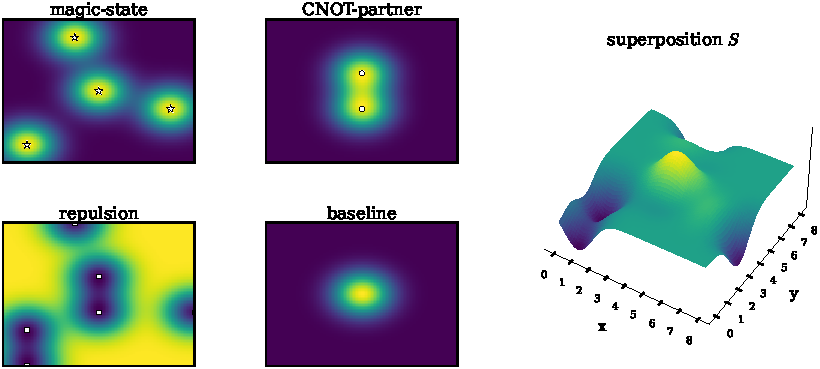
\includegraphics[width=\linewidth]{figures/gaussian_fields.pdf}
    \caption{Decomposition of the Gaussian fields for one qubit: the
    magic-state, CNOT-partner, repulsion, and baseline field families (heatmaps,
    left) and their superposition $S$ as a surface over the lattice (right).
    Markers denote the magic tiles ($\star$), the qubit's interaction partners
    ($\circ$), and already-placed patches ($\square$); the red marker on $S$ is
    its safe maximum.}
    \label{fig:fields}
    \vspace{-0.5cm}
\end{figure}


\subsection{Coarse and Fine Weighting}

The two variants differ only in how each field's weight $w$ and its
attractive/repulsive sign are read off the circuit statistics. Both use a small
set of non-negative tuned constants---\textsc{magic-high}, \textsc{magic-low} for
the magic fields and \textsc{cnot-high} for the partner fields---whose values are
fixed per regime by the sweeps of Section~\ref{sec:eval} and listed in the
repository~\cite{ftqc}.

The \emph{coarse} variant makes discrete decisions from a qubit's $T$-count $t(q)$
and its largest single-partner CNOT count $c_{\max}(q)=\max_{p}c(q,p)$: the qubit
is \emph{$T$-bound} when $t(q)>c_{\max}(q)$ and \emph{partner-driven} otherwise.
Its magic-field weight switches on only for qubits whose $T$ demand is more than
one standard deviation from the mean,
\begin{equation*}
w^{\mathrm{mag}}_q \;=\;
\begin{cases}
\textsc{magic-high}, & |t(q)-\bar t|>\sigma_t,\\[2pt]
0, & \text{otherwise,}
\end{cases}
\end{equation*}
the field being attractive if $t(q)>c_{\max}(q)$ and repulsive if
$t(q)\le c_{\max}(q)$. In the partner-driven regime it also adds an attractive
CNOT field at every mapped partner $p$ with above-average interaction
($c(q,p)\ge\bar c$), and triples the pull toward the single dominant partner
$p^{\star}=\arg\max_p c(q,p)$,
\begin{equation*}
w^{\mathrm{cnot}}_{p} \;=\;
\begin{cases}
3\,\textsc{cnot-high}, & p=p^{\star},\\[2pt]
\textsc{cnot-high}, & \text{otherwise.}
\end{cases}
\end{equation*}

The \emph{fine} variant replaces the thresholds with linear interpolation, writing
$\mathrm{lerp}(a,b,s)=a+s\,(b-a)$ for $s\in[0,1]$. For the magic fields,
\begin{equation*}
w^{\mathrm{mag}}_q =\!
\begin{cases}
\textsc{magic-high}, & \hspace{-40pt} |t(q)-\bar t|>\sigma_t,\\[2pt]
\mathrm{lerp}\!\big(\textsc{magic-low},\textsc{magic-high},\tfrac{|t(q)-\bar t|}{\sigma_t}\big), & \hspace{5pt} \text{else},
\end{cases}
\end{equation*}
attractive when $t(q)>\bar t$ and repulsive when $t(q)<\bar t$; the CNOT fields are
weighted analogously from the per-pair count $c(q,p)$ relative to $\bar c$ and
$\sigma_c$. Fine thus reacts smoothly to how far a qubit deviates from the
circuit's average resource profile, while coarse commits to a hard on/off split.

\subsection{Placement-and-Routing Loop}
\label{sec:loop}

Placement is greedy and proceeds in a single pass. We first rank qubits by
\emph{interaction importance}---a qubit's $T$-count plus its largest single-partner
CNOT count---and commit the most important first, so the mapping forms around the
qubits that constrain it most while the lattice is still empty. Because a qubit's
partner fields act only on partners that are already placed, the visiting order
matters on sparse circuits: when the CNOT interaction graph has density below a
threshold $\tau$ ($0.7$ by default) we expand placement in \emph{CNOT-BFS} order,
starting from the highest-importance qubits and visiting each interaction
neighbourhood breadth-first, heaviest partner first, so every qubit finds its
strongest partner already in place; on dense graphs, which offer no such locality,
we keep the plain importance order. For each qubit we evaluate the score $S$ of
\eqref{eq:score} on every free tile, sort the tiles by decreasing $S$, and commit
the first that doesn't violate safe passage
(Definition~\ref{def:safepassage}), adding a repulsion field there; if no tile
passes, placement reports failure.
Algorithm~\ref{alg:main} summarises the loop and Figure~\ref{fig:frames} shows the potential-field variation as
the mapping grows.

% ---- ALGORITHM: Gaussian field placement ----
\begin{algorithm}[t]
\caption{Gaussian field placement}
\label{alg:main}
\begin{algorithmic}[1]
    \Require Circuit $\C$, architecture $\A$ with magic tiles $V_{\mathrm m}$
    \Ensure Safe-passage mapping $\M$
    \If{CNOT-graph density $<\tau$}
        \State order $\Q_L$ by CNOT-BFS
    \Else
        \State order $\Q_L$ by interaction importance
    \EndIf
    \State $\M \gets \emptyset$;\; add baseline field; add magic fields
    \For{$q$ in order}
        \State build magic/CNOT field weights
        \State $S(v)\gets$ superpose fields over each free tile $v$
        \For{$v$ in tiles sorted by $S(v)$ descending}
            \If{\Call{SafePassage}{$v,q,\M$}}
                \State $\M(q)\gets v$;\; add repulsion field at $v$;\; \textbf{break}
            \EndIf
        \EndFor
        \If{no tile committed} \State \textbf{fail} (no routable placement) \EndIf
    \EndFor
    \State \Return $\M$
\end{algorithmic}
\end{algorithm}


The resulting mapping is handed to the router, which produces a routing
$\Rout$ (Definition~\ref{def:routing}). Our \emph{packing} router schedules as many
vertex-disjoint corridors per step $P_i$ as it can, prioritising gates that are
critical to the downstream schedule, and serves $T$ gates with a dedicated
strategy that reserves a corridor to the nearest free magic-state tile; a simpler
\emph{naive-critical} shortest-path router is also available. Because the mapping already
satisfies safe passage (Definition~\ref{def:safepassage}), every gate stays
reachable and the router never deadlocks---its only job is to keep $|\Rout|$ small
by packing each step densely.

The two routers differ in how they fill each step. The
\emph{packing} router proposes a few
candidate corridors for every waiting gate and then greedily commits a 
maximal mutually disjoint subset, taking gates
in order of \emph{downstream criticality} (how many of the next few layers depend
on each gate's qubits) and deferring whatever does not fit to the following step.
The \emph{naive-critical} router is the lightweight alternative: it lays down a
single shortest path per gate, visits gates in the same criticality order, and
simply defers any gate whose path would collide with one already placed.
It is cheaper but packs each step less densely, so it generally
uses more routing steps than packing. The full routers are described in the
artifact~\cite{ftqc}.

% ---- FIGURE: mapping-formation frames (single column) ----
\begin{figure}[t]
    \centering
    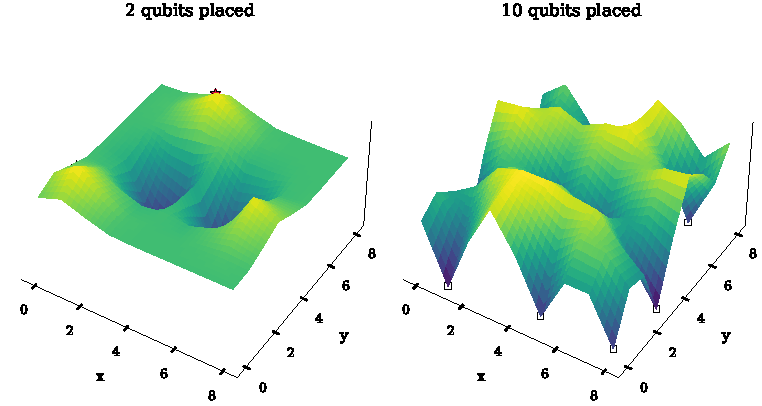
\includegraphics[width=\linewidth]{figures/gaussian_frames.pdf}
    \caption{Formation of a Gaussian-field mapping: the (per-panel normalised)
    score surface $S$ after the indicated number of qubits are committed. White
    squares are committed patches, red stars magic tiles; repulsion carves a well
    at each patch, spacing qubits apart.}
    \label{fig:frames}
    \vspace{-0.5cm}
\end{figure}


\begin{remark}
Evaluating the field for one qubit costs
$O(|V|\cdot(|V_{\mathrm m}|+|P(q)|+|\Q_L|))$, and with the lattice sized as
$\Theta(|\Q_L|+|V_{\mathrm m}|)$ tiles the whole placement is low-order
polynomial in the qubit count.
\end{remark}

% ============================================================
\section{Evaluation}
\label{sec:eval}

We ask whether a cheap geometry-aware placement routes as well as far more
expensive joint schedulers. This section describes the implementation and
benchmark suite, the baselines we compare against, and our results.

\subsection{Experimental Setup}

The method is implemented in an open-source C++20 compiler~\cite{ftqc} that parses
OpenQASM, generates the rectangular architecture and its magic-state placement,
runs the mapping of Section~\ref{sec:approach}, and routes the result with a
lattice-surgery router; the lattice dimensions are sized automatically from the
qubit count, the interaction degree, and the magic-state budget. The benchmark
suite spans \todo{$N$} circuits from three families---arithmetic
(\texttt{adder}, \texttt{multiplier}, \texttt{square\_root}), algorithmic
(\texttt{qft}, \texttt{qpe}, \texttt{bwt}, \texttt{hhl}, \texttt{factor247}), and
structured or state-preparation (\texttt{ghz}, \texttt{wstate}, \texttt{ising},
\texttt{qaoa})---with logical qubit counts from \todo{min} to \todo{max}.

We compare our (fine) Gaussian placement against two baselines. The first,
\emph{random}, scatters qubits over a sparse sublattice with $3\times3$ spacing,
which trivially satisfies safe passage (the cube condition of
Section~\ref{sec:background}), and routes it with the same router as Gaussian;
since each restart is so cheap, we run it for \todo{N} repetitions and
keep the best result, whereas the Gaussian placement is deterministic and runs
once. The second is the external WISQ compiler~\cite{wisq}. The primary metrics
are the routing-step count $|\Rout|$ (Definition~\ref{def:routing}), bounded below
by the circuit depth $\Rmin$, and the compilation time; our implementation
additionally reports the average gate parallelism and the average non-routed-gate
percentage per layer (Definition~\ref{def:layering}).

\subsection{Results}

Table~\ref{tab:results} reports the routing-step count $|\Rout|$ and compilation
time across the suite for the Gaussian method and the two baselines, and
Figure~\ref{fig:scatter} plots per-circuit $|\Rout|$ of the Gaussian method against
WISQ: points below
the diagonal favour our method, while the WISQ column of the table flags circuits
where WISQ fails or times out though the Gaussian method completes. The field
weights of Section~\ref{sec:fields} were tuned per gaussian variant (coarse or fine) 
and safe-passage strategy (cube or connectivity) 
by benchmark sweeps, with the full values provided in the project repository~\cite{ftqc}.

% ---- TABLE: main comparison (single column) ----
\begin{table}[t]
    \centering
    \caption{Routing steps and compilation time per benchmark.\\[2pt]
    ``Gauss'' is the (tuned) Gaussian ``fine'' placement,\\
    ``Rand'' is the best of \todo{N} randomized baselines. \\
    $L_{\min}$ is the circuit layer count (minimum routing steps).\\
    $|\Q_L|$ is the circuit qubit count.\\
    \todo{Fill table from CSV runs + WISQ.}
    }
    \label{tab:results}
    \setlength{\tabcolsep}{3pt}
    \scriptsize
    \begin{tabular}{l r r rrr rrr}
        \toprule
        \textbf{Circuit} & \textbf{$|\Q_L|$} & \textbf{$L_{\min}$}
            & \multicolumn{3}{c}{\textbf{Routing steps}}
            & \multicolumn{3}{c}{\textbf{Compilation time (s)}} \\
        \cmidrule(lr){4-6}\cmidrule(lr){7-9}
            & & & \textbf{Gauss} & \textbf{Rand} & \textbf{WISQ}
              & \textbf{Gauss} & \textbf{Rand} & \textbf{WISQ} \\
        \midrule
        \texttt{adder}        & 28 & -- & -- & -- & -- & -- & -- & -- \\
        \texttt{qft}          & 20 & -- & -- & -- & -- & -- & -- & -- \\
        \texttt{multiplier}   & 45 & -- & -- & -- & -- & -- & -- & -- \\
        \texttt{square\_root} & 45 & -- & -- & -- & -- & -- & -- & -- \\
        \texttt{bwt}          & 21 & -- & -- & -- & -- & -- & -- & -- \\
        \texttt{hhl}          & 10 & -- & -- & -- & -- & -- & -- & -- \\
        \texttt{factor247}    & 15 & -- & -- & -- & -- & -- & -- & -- \\
        ~~$\vdots$ & & & & & & & & \\
        \midrule
        \textbf{Mean}    & -- & -- & -- & -- & -- & -- & -- & -- \\
        \bottomrule
    \end{tabular}
    \vspace{-0.2cm}
\end{table}

% ---- FIGURE: per-circuit scatter vs WISQ (single column) ----
\begin{figure}[t]
    \centering
    \figslot{1.6in}
    \caption{Per-circuit routing step ratios: Gaussian / WISQ~\cite{wisq}.
    Points below the diagonal indicate fewer routing steps for our method.
    \todo{Generate from CSVs.}}
    \label{fig:scatter}
    \vspace{-0.2cm}
\end{figure}

% ---- TABLE: tuned Gaussian parameters per regime (full width) ----
% Currently kept in the project README ("Tuned Gaussian mapping parameters").
% To show it in the paper, remove the \iffalse ... \fi wrapper and re-point the
% "tuned per regime" sentence in sections/evaluation.tex to Table~\ref{tab:params}.
\iffalse
\begin{table*}[t]
    \centering
    \caption{Tuned Gaussian parameters by regime (weighting variant $\times$
    lattice geometry). Common to all configurations: \texttt{external\_weight}
    $=0$, \texttt{base\_gaussian\_weight}$=1$, \texttt{cnot\_low}$=0$,
    \texttt{number\_of\_magic\_states}$=-1$ (auto), \texttt{center\_circle}
    magic placement with a border margin, and naive routing with smart
    $T$-routing. ``mapped'' is the repulsion-field weight and $\kappa$ the
    confidence of \eqref{eq:sigma}; \textsc{magic-high} depends on the border
    margin $b$ (percent), while all other weights do not.}
    \label{tab:params}
    \setlength{\tabcolsep}{5pt}
    \footnotesize
    \begin{tabular}{l cccc ccccc}
        \toprule
        & \multicolumn{4}{c}{\textbf{Border-independent weights}}
        & \multicolumn{5}{c}{\textbf{\textsc{magic-high} by border $b$ (\%)}} \\
        \cmidrule(lr){2-5}\cmidrule(lr){6-10}
        \textbf{Regime} & \textbf{$\kappa$} & \textbf{\textsc{cnot-high}} & \textbf{mapped} & \textbf{\textsc{magic-low}}
            & $b{=}0$ & $b{=}5$ & $b{=}10$ & $b{=}20$ & $b{=}30$ \\
        \midrule
        \regime{coarse}{cube} & 0.999999 & 1.5 & 0   & 0              & 0               & 0.2 & 0.2 & 0.2 & 1.6 \\
        \regime{coarse}{conn} & 0.99999  & 1.5 & 2.0 & 0              & 0               & 0.2 & 0.8 & 0.8 & 0.2 \\
        \regime{fine}{cube}   & 0.999999 & 0.5 & 0   & $1^{\dagger}$  & $20^{\ddagger}$ & 3   & 1.6 & 0   & 0   \\
        \regime{fine}{conn}   & 0.99999  & 0.5 & 1.5 & 0              & 3               & 1.6 & 0.4 & 0.4 & 0.2 \\
        \bottomrule
    \end{tabular}

    \vspace{2pt}
    {\footnotesize $^{\dagger}$\,\textsc{magic-low}$=1$ for border $b\le10\%$, else $0$ (fine\,/\,cube only).\quad
    $^{\ddagger}$\,Robust argmin is $20$, but the curve is flat above ${\sim}1.6$.}
\end{table*}
\fi


\todo{Discussion, 2--4 sentences once numbers are in: (i) where the field method
beats or loses to WISQ and why; (ii) how many randomized restarts the random
baseline needs to match field placement, if ever, and at what grid-area cost;
(iii) scalability.}

% ============================================================
\section{Conclusion}
\label{sec:conclusion}

We presented a Gaussian potential-field heuristic for the placement sub-problem of
fault-tolerant compilation. The method superposes attractive magic-state and
partner fields with repulsive fields and places each qubit at the safe maximum of
the result, folding $T$-gate locality, interaction clustering, and corridor
preservation into a single fast scoring pass while safe passage keeps every
mapping routable. Implemented in an open-source OpenQASM-to-lattice-surgery
compiler and evaluated against a randomized-restart baseline and the WISQ
compiler, it \todo{state the headline result once the tables are filled}.

The method has four main limitations. First, placement is static and single-pass:
once a qubit is committed, the mapper does not revise earlier choices in response
to congestion revealed during routing. Second, the field weights are hand-tuned
rather than learned or jointly optimized, which may limit generalization across
workload classes. Third, the heuristic optimizes initial-placement quality and
downstream routing steps, but does not explicitly co-optimize architecture-level
bottlenecks such as dynamic factory throughput, logical-error accumulation, or
event-driven resource contention~\cite{kan2025sparo,bharadwaj2026qomet}. Fourth,
our experimental comparison is deliberately narrow---a randomized baseline and
WISQ---rather than against topology-aware or architecture-aware
compilers~\cite{zhou2026topols,kan2025sparo}. These limitations are consistent
with the broader finding that no single lattice-surgery compilation family is
universally optimal, the preferred strategy depending on circuit density,
logical-qubit count and $T$ fraction~\cite{leblond2025comparison}.

These limitations point to natural extensions: coupling placement to router
feedback so the field adapts online to observed congestion; replacing hand-tuned
coefficients with workload-conditioned or learned parameters; and evaluating the
field placement as an initializer for stronger downstream optimizers---including
topology-aware compilers and architecture-aware
schedulers~\cite{zhou2026topols,bharadwaj2026qomet}---or against emerging
alternatives to static place-and-route such as movable logical
qubits~\cite{herzog2025movable}. More broadly, our results suggest practical value
in lightweight, interpretable front-end mappers: a deterministic field-based
placement occupies a useful middle ground, capturing the key geometric constraints
of lattice-surgery execution at very low computational cost while serving as a
strong standalone baseline and a possible initialization layer for more expensive
optimization flows. Seen this way, the magic-state--aware attractive fields are a
local proxy for the broader class of workload-dependent resource bottlenecks
identified in recent fault-tolerant resource
analyses~\cite{ogorman2017factories,leblond2025comparison}.


\section*{Acknowledgements}
Acknowledgements to the funding entity omitted for blind review.

% ── References ───────────────────────────────────────────────
\bibliographystyle{IEEEtran}
\bibliography{bib}

\end{document}
